\chapter{Challenges}

% Clustering introduction, what is it, how does it work?
% Clustering nodes with mouse
% Cluserting with regex
% Useful naming of nodes
% Avoiding false dependencies

Clustering in this paper is the action of taking a set of nodes removing them from the graph and replacing them with a single composite node. An example of this is in
% TODO make figure
Figure~\ref{fig:} where you can see the nodes x, y, z have been clustered to create the composite node named `bananas'. Our focus in this paper is the way users interact with and create composite nodes, we aim to describe a set of features that allows users to effectively and confidently use composite nodes in an effective manner.

From this task of clustering a series usability and technical challenges arise. Mainly the interface for allowing users to cluster, the automatic naming of composite nodes and issues resolving false dependencies caused by clustering. Each of these issues is described in greater detail beolow.

\section{User defined clusters}
\label{sec:user_defined_clusters}

As mentioned above, our focus is to allows users to effectively use clusters. The first method we implemented allows the user to ctrl+click multiple nodes and select the group function from a list of contexual commands (this process is described in
% TODO reference section about interfaces.
greater detail in Chapter~\ref{cha:initial_interface}). This process is however limited to allowing users to group a small amount of nodes and in usability studying users quickly become frustrated even having to group more than three or four nodes via this method.

The challenge is how to create a method for allowing users to cluster a large number of nodes without losing the fine grained control of the above process. We decided to implement a naive search function that runs a regex query on all the properties of a node and hilights any nodes with matching properties.

Future challenges involve allowing users to search for all nodes that match one regex but not another. It would also be useful to only match searches on particular properties of a node, for example a user may only want to match their search on \textit{author} of a node (assuming that property exists\footnote{Breifly discussed in the introduction, the PROV standard allows an arbitraty number of key value properties to be attributed to a node.}). Many users during usability studying requested the ability to cluster all the children of a node, extending from this it would also be useful to allows uers to cluster based on a nodes relationships with other nodes, for example ``Cluster all nodes that match the following regex \texttt{X-tweets|query-X-Time} and are not derived from \texttt{TwitterFeed-time-3}.

Possiblty the biggest challenge in this section would be that of paramaterised clustering. Where a single action by the user would create mutliple clusters. A common clustering we found while studying participants was selecting the entity and the actitvity and creating a composite node of them. In Figure~\ref{fig:search1} they would cluster \texttt{[X-tweets-1, query-X-time-1]}, \texttt{[X-tweets-2, query-X-time-2]} and \texttt{[X-tweets-3, query-X-time-3]} into seperate composite nodes. This would be an ideal use of a paramaterised language that would allow the user to ``group all X-tweets with their corosponding query-X-Time'', however creating a language that is both powerfl and easy to learn and use will be quite a challenge.

A possible future endevour would be automation of clustering. Where the application woudl suggest clusterings based on previous provenance workloads. It may then group together infrequently accessed nodes to make it easier to access infrequently used nodes.

\section{Naming composite nodes}
\label{sec:naming_composite_nodes}

When a composite node is created it must be given a name. In an early version of the ProvOwl system nodes where given short random alhpa-numeric names. We found that this soon made the graph incomprehensible and relied on the user manually 
% TODO Reference interface -> rename section
renaming (described in Section~\ref{sec:}) each node in order for the graph to be usable. 

Ideally an interface would give clusters a name describing the nodes inside of it. However htis requires on domain level knowledge and would even require models of the user and what information is important to them. For example say that the nodes \texttt{sunflower}, \texttt{daphodil} and \texttt{poppies} where to be clustered. Naively it would be useful to name the cluster \textit{plants}, however if the user was a plantologist
% TODO find real name of plantologists
this might be too vague and they would instead prefer to have a node labelled \textit{flowers} or with the root genius of the plants. 

In some fields this problem has been solved by limiting the number of unkowns. If you create a new folder on an iPhone it is automatically named with a label approproate to the applications inside of it. A folder full of photography apps may be labelled \textit{Photography}. However this differs from the problem we are trying to solve in a variety of ways. Firstly the number of possible labels is limited to the categories in the Apple app store, this creates a finite set of possible options. Secondly, when an application is uploaded to the app store the author publishes metadata with it such as the category of the app. Using this metadata makes it much easier to name clustered items. Having the same level of metadata in provenance files could be accomplished by having tags associated with each node. These tags could then be used to effectively name a cluster simply by selecting the most used tag from the group of nodes to be clustered.

Our currently, still simple approach uses the name of the node in the cluster closest to the root with the text ``group'' appended to the end.

\begin{figure}[h]
	\centering
	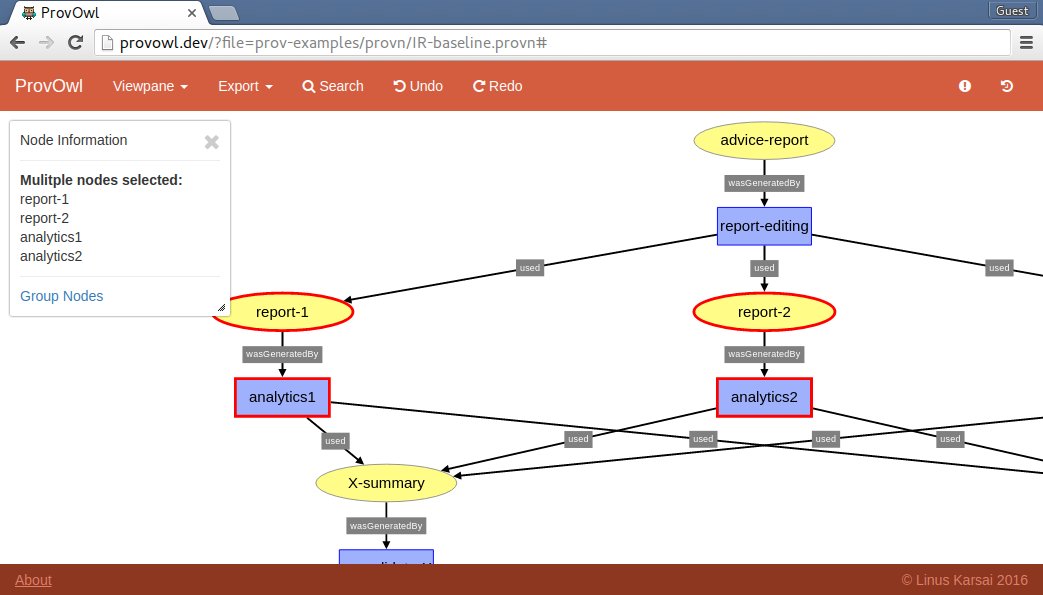
\includegraphics[width=\linewidth]{naming1}
	\caption{Using the \textit{IR-baseline} example the user has selected four nodes for grouping, essentially those related to \texttt{report-1} and \texttt{report-2}.}
	\label{fig:naming1}
\end{figure}
\begin{figure}[h]
	\centering
	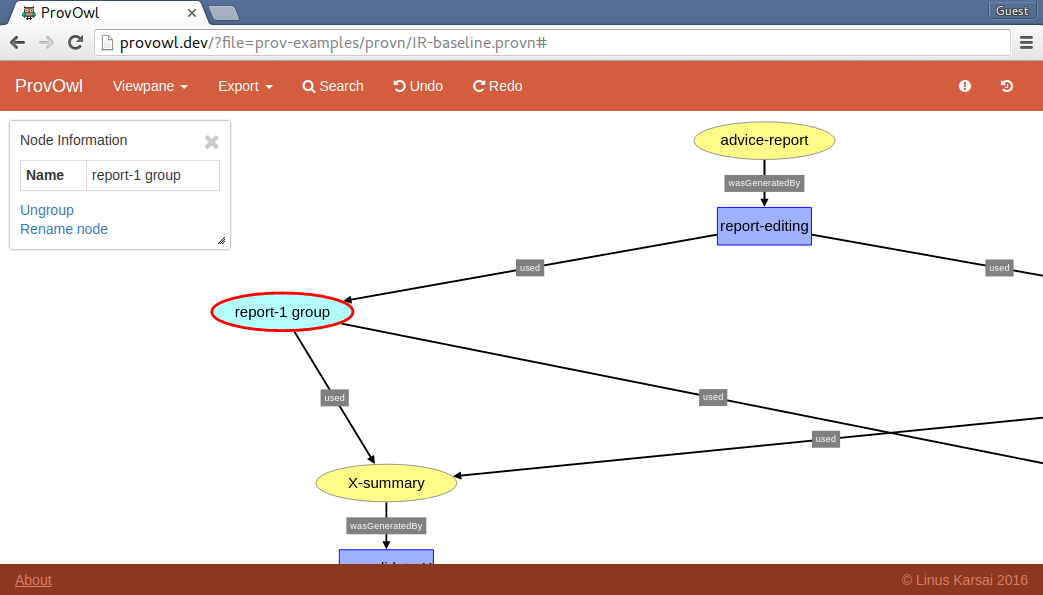
\includegraphics[width=\linewidth]{naming2}
	\caption{When clusterint the four nodes selected in Figure~\ref{fig:naming1} ProvOwl creates a composite node using the name of the node closest to the root (in this case breaking a tie by alphabetical order).}
	\label{fig:naming2}
\end{figure}
\clearpage

\section{False Dependencies}
\label{sec:section_name}

In essense clustering is a simple type of graph rewriting that creates an abstraction of a graph and in turn simplifies deatails. This can cause some anomolies such as false dependencies, circular dependencies and mislabelled relationships. 

A false dependency is when a clustering in the graph has caused a newly implied line of linage that falsly suggests that one enetity had influence upon another. This is in violations of the main assumption that provenance records the factual history of data derivation. The opposite of this, removing a dependency, is not such an issue because it is understood that the ability to observe data trasnformations is limited so therefore all provenaance graphs are expected to be partially incomplete. In Figure~\ref{fig:falsedependencies} you can see a simple example that shows a false dependency caused by joinging nodes \texttt{B1} and \texttt{B2} together. It creates a new line of lineage that falsly implies \texttt{A1} and \texttt{A2} where influenced by \texttt{C1} and \texttt{C2}. Technical consequences of false dependencies also include unnecessary checks and recomputation when revisiting dependent entities to reflect corrected or changed source data. For example if the data in \texttt{C1} was found to be incorrect it would be necessary to follow the lineage up to find what entities need to be recomputed, in the case of Figure~\ref{fig:} (B) this would include both \texttt{A1} and \texttt{A2}.

\begin{figure}[H]
	% TODO fix graph
  \begin{subfigure}[t]{0.5\textwidth}
    \centering
    \begin{tikzpicture}
      \node[main node] (root) {root};
	  \node[main node] (A1) [below left of=root] {A1};
      \node[main node] (A2) [below right of=root] {A2};
      \node[main node] (B1) [below of=A1] {B1};
      \node[main node] (B2) [below of=A2] {B2};
      \node[main node] (C1) [below of=B1] {C1};
      \node[main node] (C2) [below of=B2] {C2};
      \path (A1) edge node[left] {used} (B1);
      \path (A2) edge node[left] {used} (B2);
      \path (B1) edge node[left] {used} (C1);
      \path (B2) edge node[left] {used} (C2);
      \path (root) edge node[left] {used} (A1);
      \path (root) edge node[right] {used} (A2);
    \end{tikzpicture}
    \caption{A small example provenance graph that shows two main lines of lineage from the root.}
  \end{subfigure}
  ~
  \begin{subfigure}[t]{0.5\textwidth}
    \centering
    \begin{tikzpicture}
      \node[main node] (root) {root};
      \node[main node] (A1) [below left of=root] {A1};
      \node[main node] (A2) [below right of=root] {A2};
	  \node[main node, group] (CB) [below = 2cm of A1] {B group};
      \node[main node] (C1) [below = 5cm of A1] {C1};
      \node[main node] (C2) [below = 5cm of A2] {C2};
      \path (CB) edge node[left] {used} (C1);
      \path (CB) edge node[right] {used} (C2);
      \path (A1) edge node[left] {used} (CB);
      \path (A2) edge node[right] {used} (CB);
      \path (root) edge node[left] {used} (A1);
      \path (root) edge node[right] {used} (A2);
    \end{tikzpicture}
	\caption{Nodes \texttt{B1} and \texttt{B2} are clustered into the \texttt{B group} composite node.}
  \end{subfigure}
	\label{fig:falsedependencies}
	\caption{When \texttt{B1} and \texttt{B2} are clustered together it creates a false line of lineage that suggests that \texttt{A2} was influenced by \texttt{C2}, this is known as a false dependency.}
\end{figure}

Circular dependencies are another animality that may also occur. This means that the graph is no longer a directed acyclic graph and can cause issues with algorithms that assume the graph is acyclic. It is also in direct violation of the constraints defined in the PROV-CONSTRAINTS W3C document~\cite{}. Figure~\ref{} shows an example of a circular dependency between \texttt{Fitness-Summary group} and \texttt{Summarize}.

The last anomaly that we noticed was that of mislabelled relationships. The labels used to label relationships are specific to the types of nodes the edge is connecting. For example an Entity \textit{was generated by} and Activity, or an Activity was \textit{used} by an Entity. Clustering creates a fourth node type in conjunction with the existing three (Activity, Entity and Agent) and doesn't have any limitation to the labls that can be used on relationships associated with it. This can be confusing to users and can also reveal information about nodes inside a cluster (a used relationship to a cluster node says that there's an entity inside of it). There's also the case of when clustered nodes created multiple relationhips to nodes in common, which relationship label should be picked to represent the relationship? At the moment ProvOwl arbitarily selects one. 

A theoretical formulation of provenance abstraction by clustering has been proposed in~\cite{Missier2014} to discuss this and other problems that occur in clustering, along with simple algorightms for grouping arbitary sets of nodes. In essense the work showed that to avoid false dependencies one must compute a \textit{closure} operation that extends the user-selected nodes with all other nodes that sit on any path amongst these inisial clustering nodes. Combining this work with our user-oriented provenance navigation system can lead to a working correct clustering mechanism. Expanding on the work of this interface to help the user cluster without creating graph anomolies is a challenge we hope to tackle in the future.
